\documentclass[11 pt]{article}

\usepackage{graphicx}
\usepackage[export]{adjustbox}
\usepackage{caption}
\usepackage{subcaption}
\usepackage{setspace}
\usepackage{hyperref}
\setstretch{1.25}

\begin{document}
\begin{titlepage}
\begin{center}
\huge{\bfseries{Project Report:}}\\
[2mm]
\huge{\bfseries{Dental Clinic Management System}}\\
Version 2.0 : Laboratory Exercise-03\\
\vskip 0.2in
\large{\bfseries{Front-End Development:}}\\
Prince Ngema (754774)\\
Luyanda Makhoba (834867) \\
\large{\bfseries{Back-End Development:}}\\
Takatso Molekane (569869)\\
Tholithemba Mngomezulu (1512124)\\
\end{center}
\end{titlepage}
\tableofcontents
\newpage
\section{Introduction}

\subsection{Purpose}
This document serves to describe the processes undertaken in the inception of the Dental Clinic Management system software project. The purpose of this document is to provide a detailed description of the DCMS ,a web application.It will give in detail the purpose of the system, features of the system and the constraints under which the system will operate. An outline of what the software aims to do at each stage, ie problem to be solved.
\subsection{Problem Statement}
Managing a dental clinic may be cumbersome at times, the paperwork that the receptionist have to do and the time patients have to spend waiting in queue is excessive. DCMS is system that will remedy this situation by allowing multiple patients at the same time\\
Hard copy files stored in cabinets pose a security threat since it is possible for unauthorized personnel to gain access because of negligence. The system will allow for the use of username and passwords, a secure measure that ensures that only permitted users can see and do certain tasks. Where in the contrary, files can easily fall into the wrong hands, be tampered with or lost.\\
Human error in the collection and capturing of all data occurs where patients either fill in their details incorrectly or the receptionist captures the data wrongly. DCMS will allow for data validation to occur, where the user will be alerted immediately if any data is incorrect or missing,ensuring the data is consistent in the database.\\
Paper files are hard to back up, the database storing capabilities adopted by DCMS will offer the ability to backup all data. \\
The automation of calculations and instantaneos syncing of events will allow for a well integrated clinic with real time updates and time saving processing.\subsection{Project Objectives }
The software is aimed at replacing manual paper systems that currently exists at a dental clinic.Users will remotely have access to relevant services based on requirements.The project objectives are :
\begin{itemize}
\item reduce the paperwork the receptionist have to do on daily basis
\item cut the amount of waiting time in queues
\item ensure and protect patient's privacy
\item reduce human error in capturing data
\item reduce paperwork for doctors
\end{itemize}
\subsection{Stakeholders}
Anyone that is influenced by or influences a project is a stakeholder. There are two types of stakeholders , internal and external stakeholders.
\begin{itemize}
\item \textbf{External}
\begin{itemize}
\item Patients\\
Patients are able to make appointments and view their bill
\item Dentist\\
Dentists can login ,view and set their own schedule of appointments. Write out a prescription for a patient and view a patient's profile(medical record).
\item Receptionist\\
receptionist logs in with their username and password, views and manages appointments, performs day open and close activities. He also sends reports to admin and help with registering those patients who that are having problems with registering.
\item Admin \\
The administrator has the authority to add or remove a doctors and receptionist.He grants permission to receptionist and dentists the authority to view and generates report.He also has the authority to add or delete patients from system. He also manages the system
\end{itemize}
\item \textbf{Internal}
\begin{itemize}
\item Scrum team \\
responsible for developing the software
\item Product owner\\
someone in charge of the entire project
\item Scrum master \\
The link between the scrum team and the product owner(project manager)
\item Equipment suppliers \\
They supply the hardware needed for the operation of the system.(i.e) Computers
\end{itemize}
\end{itemize}
\subsection{Scope}
DCMS (Dental Clinic Management System) is a web application that provides support for managing the services of a small dental clinic.
\subsubsection{Software Benefits and Objectives}
The software is aimed at replacing manual paper systems that currently exists at a dental clinic.
Users will remotely have access to relevant services based on requirements.
Having a digital filing system will reduce human error by having text validations before data is captured. Having database will allow for backups.

\subsection{Definitions,Acronyms and Abbreviations}
\begin{tabular}{|p{3cm}|p{9cm}|}
\hline
\textbf{Term} & \textbf{Definition}\\
\hline
DCMS & A Dental Clinic Management System application\\
\hline
User & Anyone who will be interacting directly with the system..\\
\hline
Netbeans & an integrated development environment for java\\
\hline
Java & A general-purpose computer-programming language that is concurrent, class-based,object-oriented\\
\hline
PHP & Hypertext Preprocessor is a server-side scripting language designed for web development. \\
\hline
Json & JavaScript Object Notation is an open-standard file format that uses human readable text to transmit data objects consisting of attribute-value pairs and array data types \\
\hline
\end{tabular}

\subsection{References}
\begin{itemize}
\item
IEEE Recommended Practice for Software Requirements Specifications
\item
https://www.bmc.com/blogs/software-requirements-specification-how-to-write-srs-with-examples/ (Accessed Aug 2018)
\item
Zainab Murtadha- Dentist Web Based Patient Information System and Services in Cloud
\item
Virtual Medical Home SRS-Bapuju Institute
\item
https://krazytech.com/projects
\end{itemize}
\newpage



\section{Software Requirements Specifications}

\subsubsection{Product perspective}
DCMS will enable patients to book or make appointment and the output will the be date and time in which it is inline with the Doctors schedule. System will
also provide a clear schedule which allows patients to see
which Doctor is available at a particular slot. Who ever
will be using the system has to go through registration
first if he/she is first time user or login by providing
username and password to access the DCMS.The system allows patients to request their bill and the patient can view or print the through system.
\subsection{Product Functionality}
\textbf{Front End tasks:}
This involves the making of User Interfaces. These are the screens that the users will be seeing when using the system.
\begin{itemize}
\item
Create Patient(Input will be patient details)
\item
Log in(Username and Password)
\item
Create Appointment(PatientId and Date/Time)
\item
Create Bill(PatientID, DoctorID and Consultation Details)
\item
View Schedule(DoctorID and Date/Time)
\item
View Bill(PatientID)
\end{itemize}
\textbf{Back End tasks:}
\begin{itemize}
\item
Create Database with table and entities as listed in ERD
\item
Use back-end frameworks to build server-side software. PHP and JSON
\item
Cloud computing integration-Allowing Database to be accessed remotely.
\end{itemize}

\subsubsection{Existing System}
The present system is manual based. It involves paper work in the form of maintaining files, making appointments and billing.The manually based system has the following disadvantages:
\begin{itemize}
\item
it is a limited system.
\item
looking for a patient's file may take a long time
\item
patients have to queue to make an appointment
\item
There is no backup files.
\item
files are prone to damage.
\item
editing file problems.
storage space may be limited.
\item
Patient's personal information is not protected, it can be accessed by anyone.
\end{itemize}
\begin{figure}
\clearpage
\centering
\begin{subfigure}{.6\textwidth}
\centering
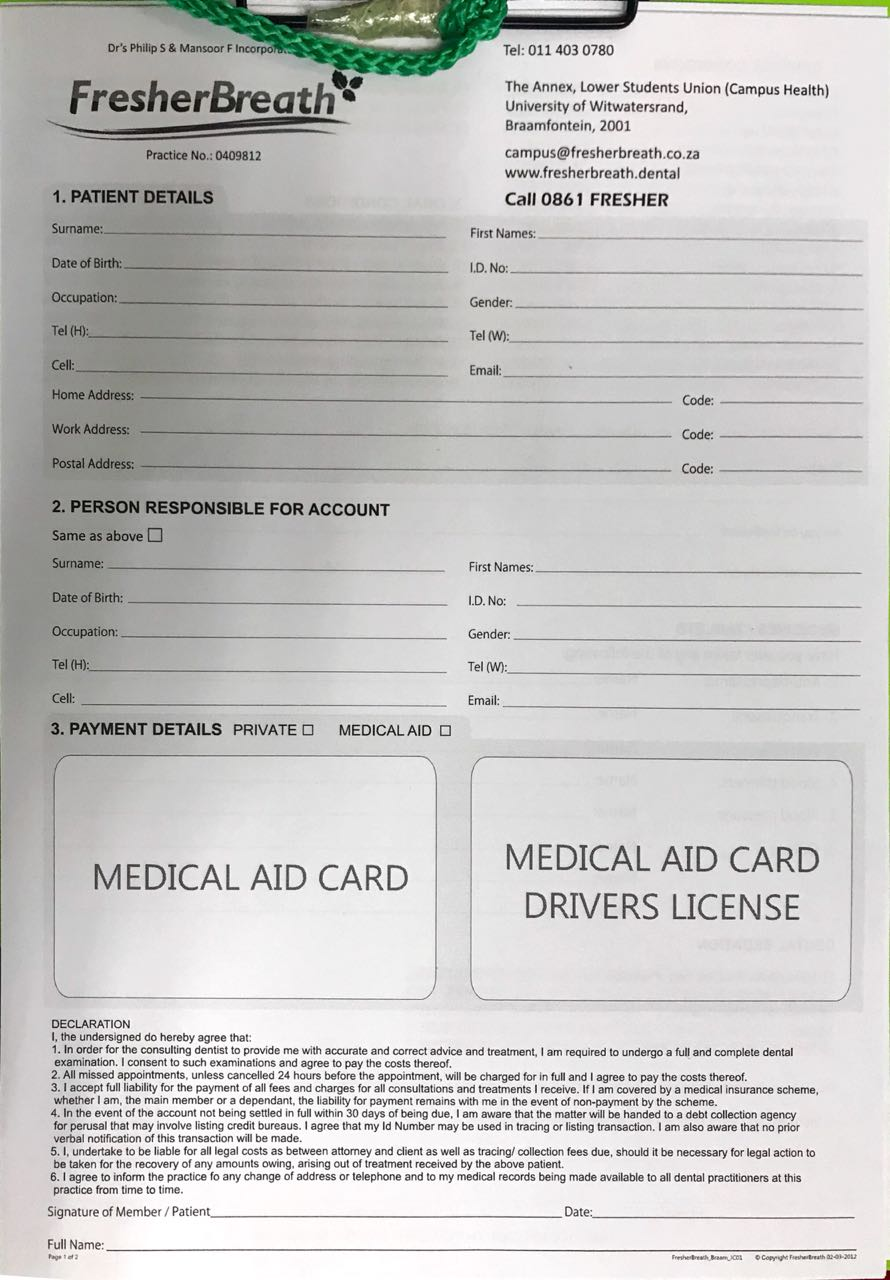
\includegraphics[width=.95\linewidth, left]{new_patient_paper_form.jpeg}
\caption{Patient personal details}
\label{fig:sub1}
\end{subfigure}%
\begin{subfigure}{.6\textwidth}
\centering
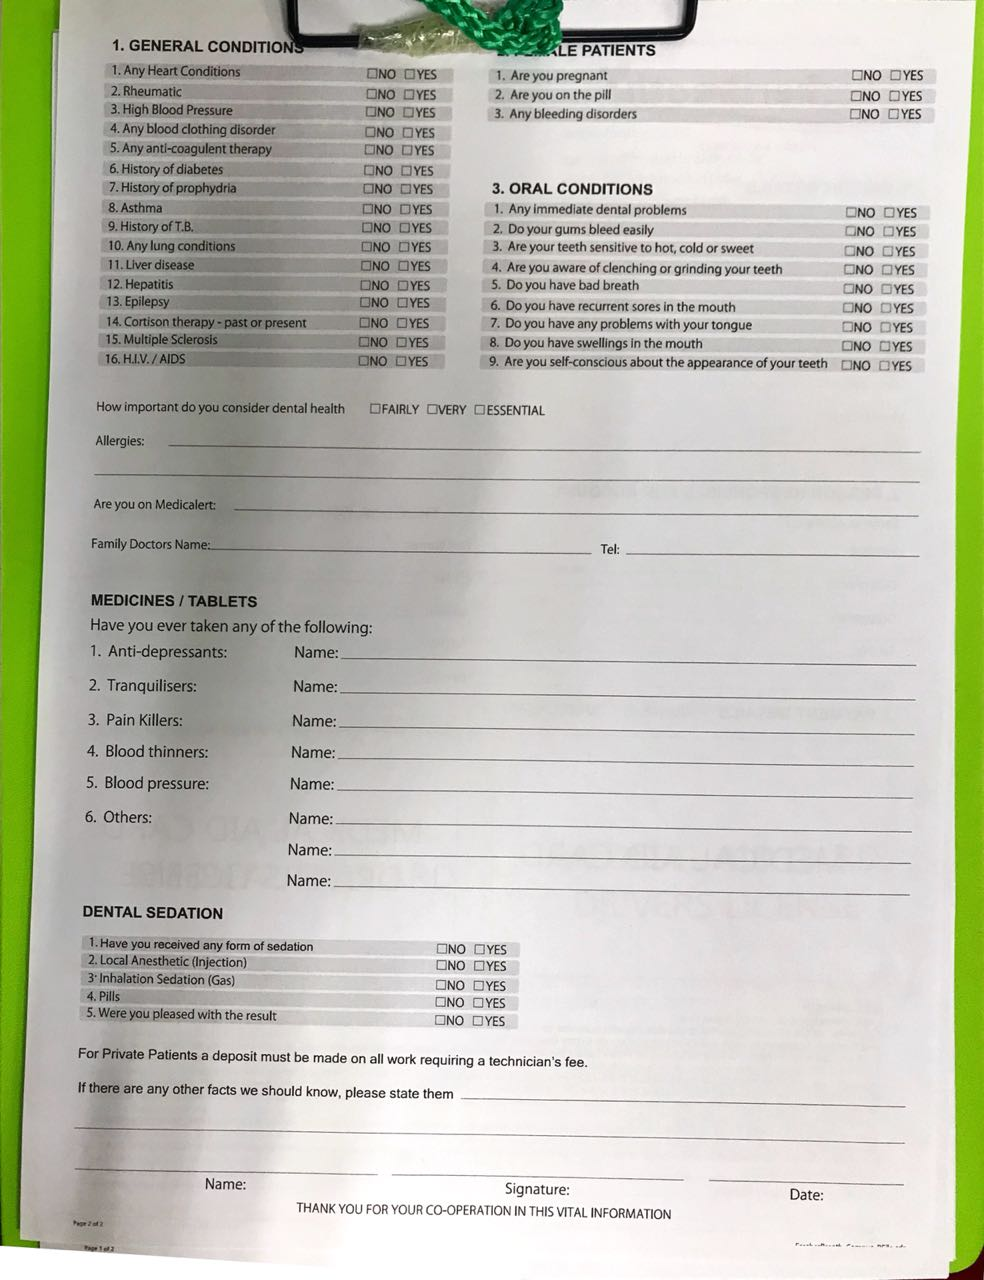
\includegraphics[width=.95\linewidth]{patient_paper_form_med.jpeg}
\caption{Medical details}
\label{fig:sub2}
\end{subfigure}
\caption{Paper forms to be replaced}
\label{fig:test}
\end{figure}

\subsubsection{Proposed System}
DCMS is an automated system that can be accessed via the internet.It has the following advantages.
\begin{itemize}
\item
Easy to store and search for files.
\item
Patients can make appointments online and avoid long queues.
\item
Each patient has a profile that can only be accessed by authorized users i.e(doctor or receptionist).
\item
The system can be accessed remotely.
\end{itemize}
\subsection{Usability}
\subsection{Assumptions and dependencies}
\begin{itemize}
\item
The receptionist and dentist all have computers that they can use at the clinic that can also offer support to patients that need the hardware or technical support.
\item
Assume financial management has instant payments notification in place. This is to allow the system to receive information on payments so that updates can be made on the respective patients bill.
\end{itemize}
\newpage
\section{Project Design and Architecture}
\subsubsection{Architecture}
\begin{figure}[h]
\centering
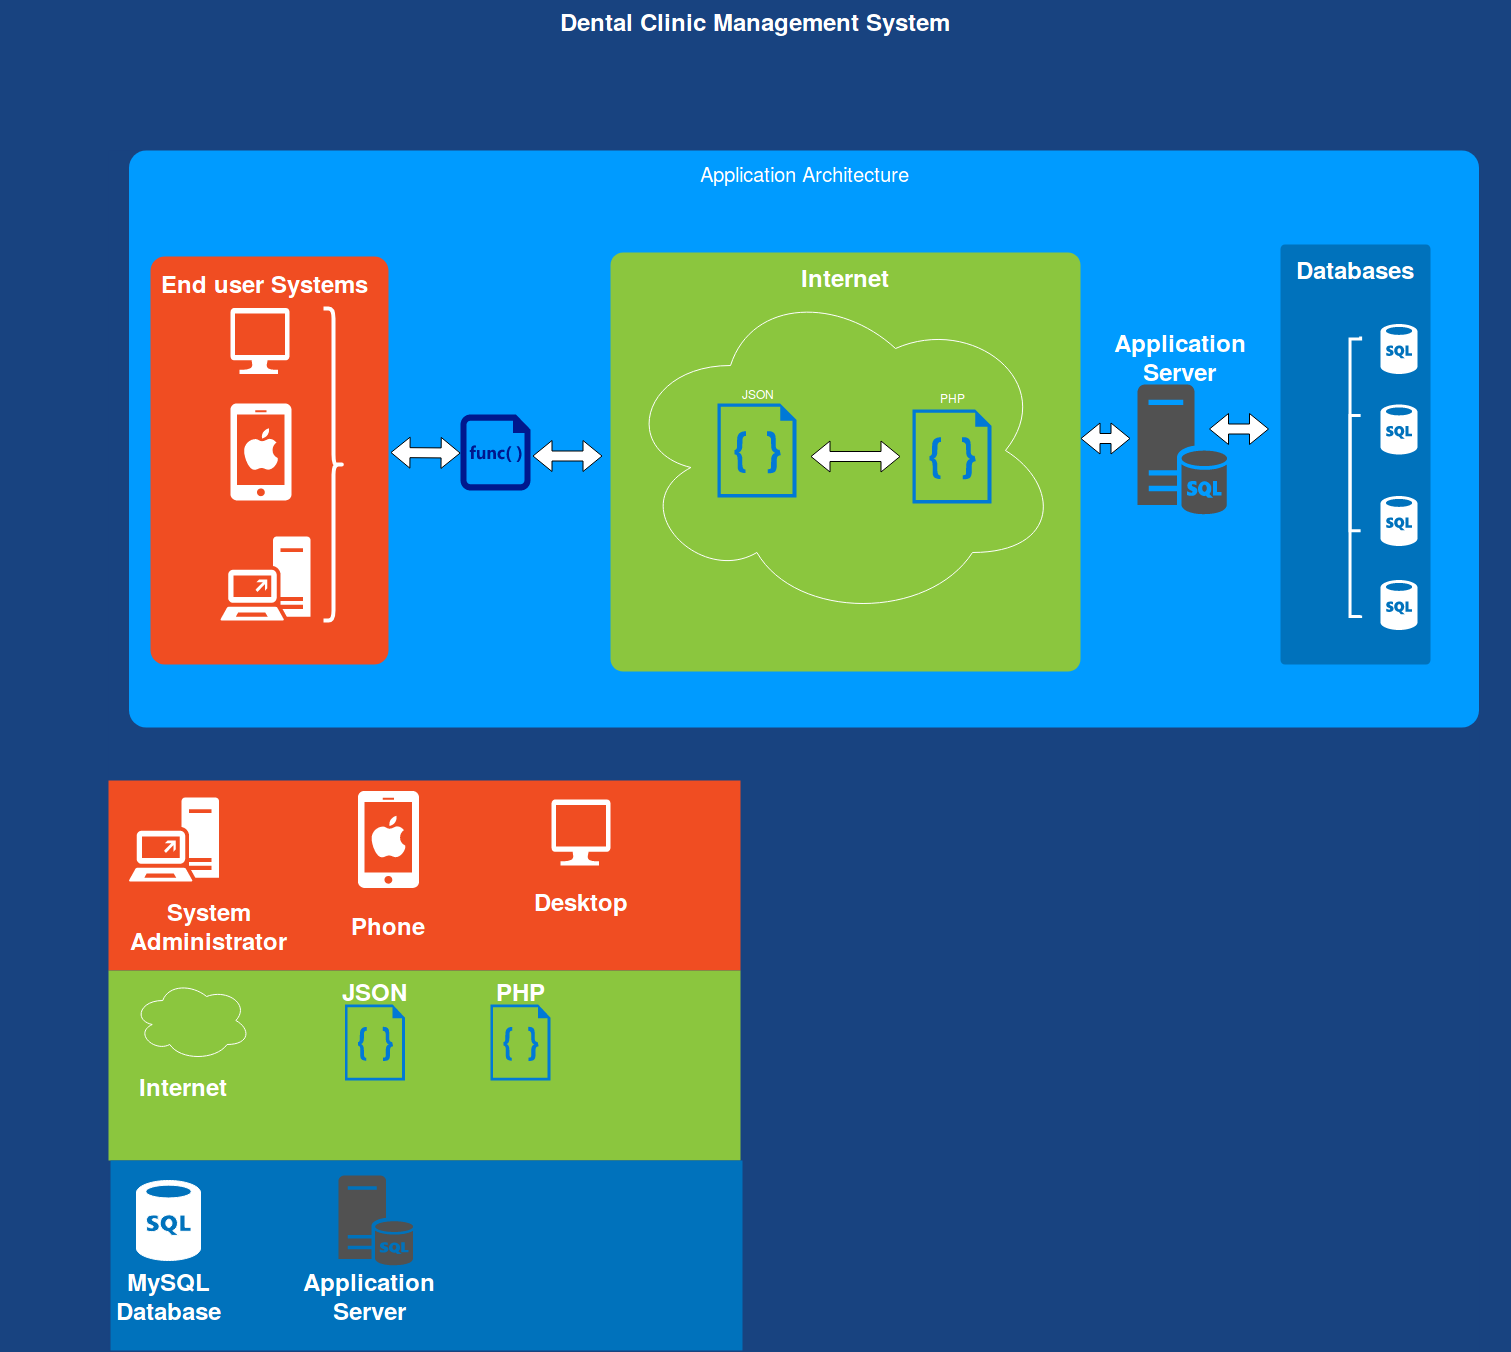
\includegraphics[width=1.2\linewidth]{architecture.png}
\caption{architecture}
\end{figure}
\begin{figure}[h]
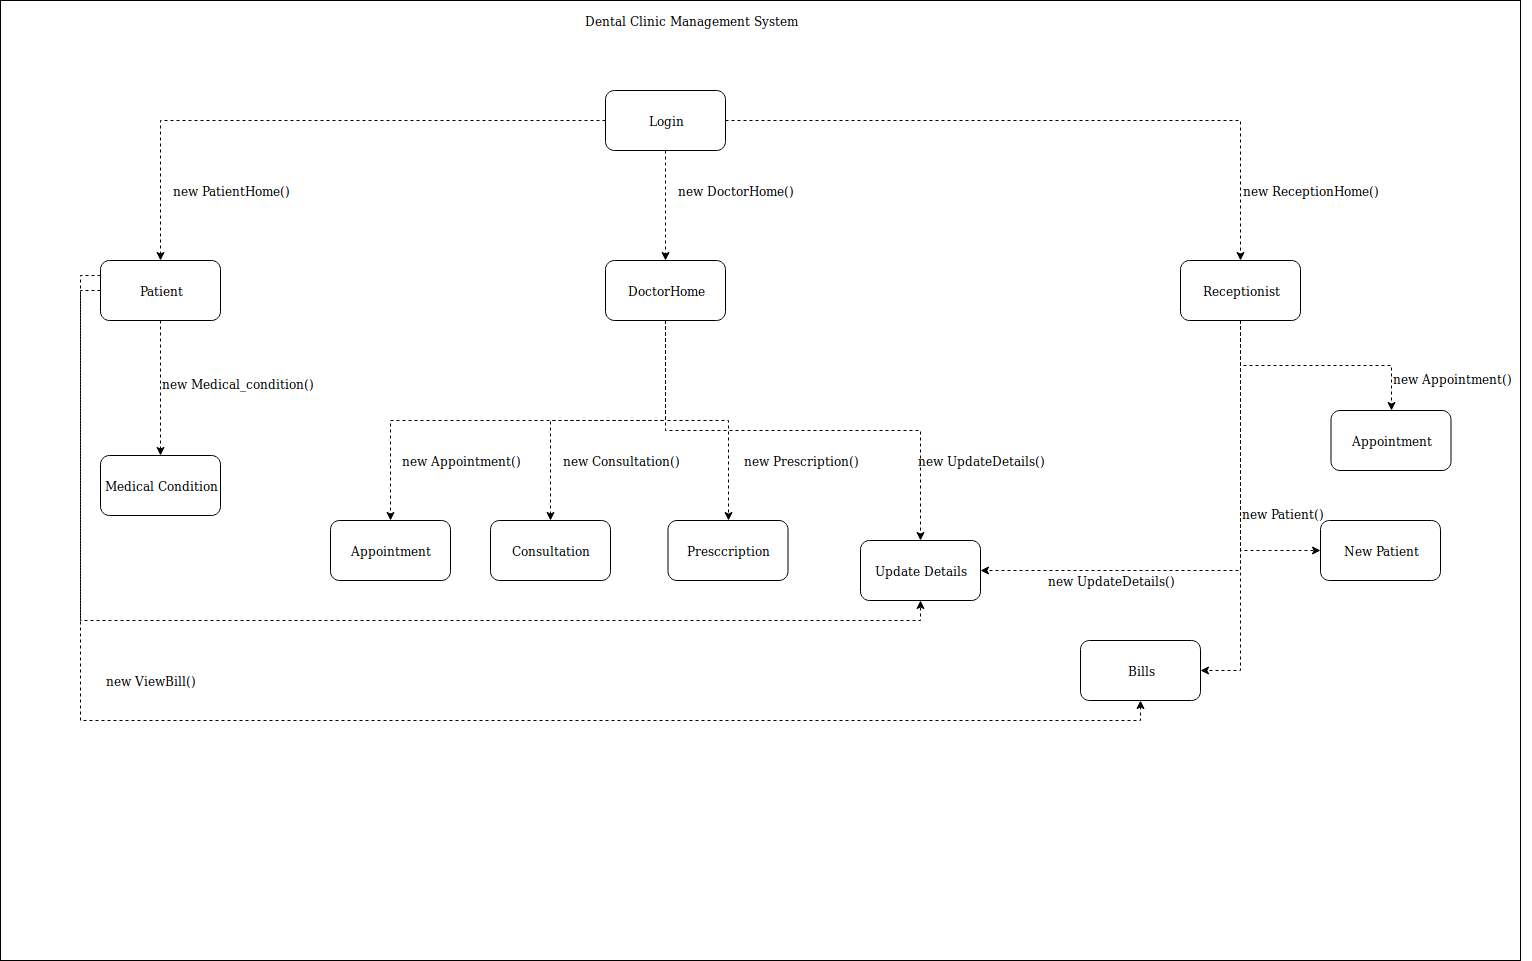
\includegraphics[width=1.2\linewidth, left]{Logical_view.png}
\caption{DCMS login}
\label{fig:login}
\end{figure}
\begin{figure}[h]
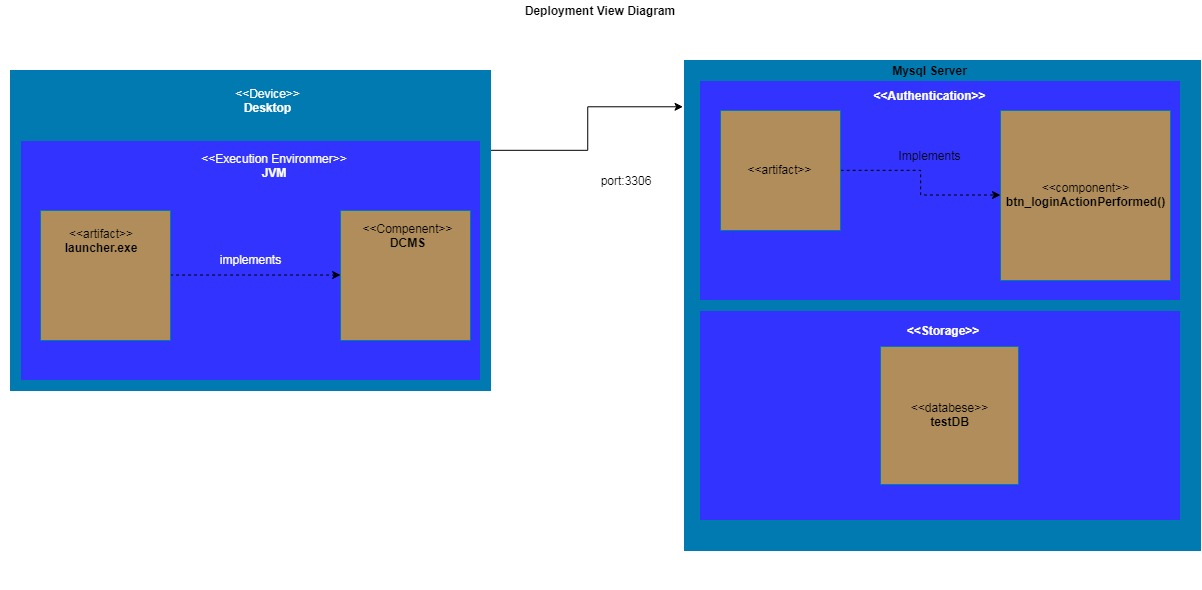
\includegraphics[width=1.2\linewidth, left]{deployment_view_diagram.png}
\caption{DCMS login}
\label{fig:login}
\end{figure}
\newpage
\subsubsection{Implemented Database Tables}
\begin{figure}[h]
\centering
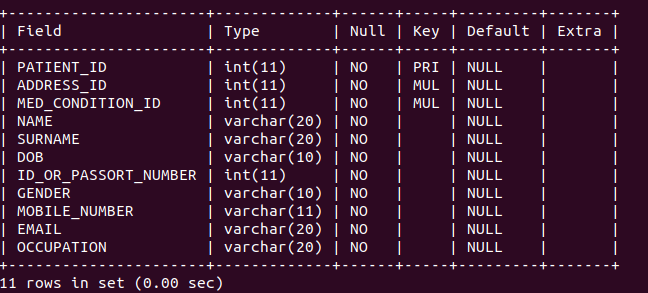
\includegraphics[width=0.8\linewidth]{PATIENT_TABLE.png}
\caption{Patient Table}
\end{figure}
\begin{figure}[h]
\centering
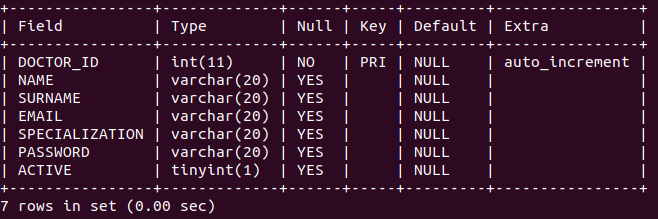
\includegraphics[width=0.7\linewidth]{DOCTOR_TABLE.png}
\caption{Doctor Table}
\end{figure}
\begin{figure}[h]
\centering
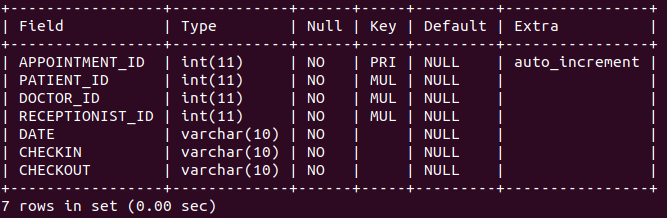
\includegraphics[width=\linewidth]{APPOINTMENT_TABLE.png}
\caption{Doctor Table}
\end{figure}
\subsubsection{Entity Relationship Diagram}

\begin{figure}[h]
\centering
\includegraphics[width=\linewidth]{"Dentist ERD".png}
\caption{DCMS-ERD}
\label{fig:ERD}
\end{figure}
\subsubsection{Software Tools}
\begin{itemize}
\item
Database Server: Microsoft SQL Server
\item
Client: Any web browser
\item
Programming Language:Java
\item
Development Tools:Netbeans IDE 8.2
\end{itemize}
\subsubsection{Hardware Requirements}
The supported Operating Systems:
\begin{itemize}

\item
\textbf{Microsoft Windows Vista SP1/Windows 7 Professional:}
\begin{itemize}
\item
Processor: 800MHz Intel Pentium III or equivalent
\item
Memory: 512 MB
\item
Disk space: 750 MB of free disk space
\end{itemize}
\item
\textbf{Ubuntu 9.10:}
\begin{itemize}
\item
Processor: 800MHz Intel Pentium III or equivalent
\item
Memory: 512 MB
\item
Disk space: 650 MB of free disk space
\end{itemize}
\item
\textbf{Macintosh OS X 10.7 Intel:}
\begin{itemize}
\item
Processor: Dual-Core Intel
\item
Memory: 2 GB
\item
Disk space: 650 MB of free disk space
\end{itemize}
\item
\textbf{Smartphone Requirements:}
\begin{itemize}

\item
Android running OS 4.0+
\item
iPhone running iOS 8+
\item
Windows Phone 8.1+
\end{itemize}
\end{itemize}
\subsection{Business Rules}
\begin{itemize}
\item
Before a user can log in, they are required to be an existing user on the System. Existing users access the system (log in) using username and password.
\begin{itemize}
\item
New Dentists and Receptionist's require an Administrators authorization to be registered on the system.
\item
A new patient is required to enter their personal and medical details.
\end{itemize}
\item
An Appointment must be booked by the patient. They have the options of doing so telephonically(Where the receptionist will be the one capturing the appointment) or engaging directly with the system. Booking of an appointment requires viewing the relevant dentist's schedule to identify available slots.
\item
A Dentist can view their schedule. This means viewing all the appointments that have been booked for the doctor and displayed as of their requirement either Daily,Weekly or Monthly schedule calendar view.
\item
A consultation is created by a dentist. This follows the arrival of a patient for their appointment and discussions or dental procedures are conducted and recorded. A consultation can also be recorded for a patients failure to arrive for an appointment without cancelling. This consultation type is labelled as missed appointment.
\item
Generating Bill follows a consultation, this is where all the costs of the medical procedure are recorded. This may also include the recording of a missed appointment charge.
\item
Authorization is done by an administrator. This is required when new a receptionist or dentist is created. Similarly so when it will be updated or deleted.
\end{itemize}
\subsubsection{Use Cases}
\begin{tabular}{|p{3cm}|p{9cm}|}
\hline
\textbf{Actor} & \textbf{Description}\\
\hline
\textbf{Receptionist} & May assist patient with registration and booking, should they require assistance.\\
\hline
\textbf{Administrator}& Administrator is responsible for Doctors registration and other issues that directly related to the system like update or archive if necessary.\\
\hline
\textbf{Patient}& Patient may directly interact with the system during registration or booking process, depending on the patient's level of of computer literacy\\
\hline
\textbf{Doctor}& May set appointment with the patient, depending on patient's problem \\
\hline

\end{tabular}
$\_$
\\\\\\

\begin{tabular}{|p{3cm}|p{4.5cm}|p{4.5cm}|}
\hline
\textbf{Use Case} & \textbf{Description} & \textbf{Related Use case and Relationships} \\
\hline
\textbf{Create Patient} & Patient or the Receptionist will interact with this use case. Step involved in this use case is entering demographic data. &\\
\hline
\textbf{Read Patient}& This use case will be used when accessing a patient's data.This includes when making appointment bookings and generating bills & Invoked by the Update Patient use case. $\textless\textless$include$\textgreater\textgreater$ relationship.\\
\hline
\textbf{Update Patient}& The Receptionist or Patient will mainly interact with this use case. It will be accessed to update a Patient's demographic data & This use case invokes the Read Patient use case. $\textless\textless$include$\textgreater\textgreater$ relationship\\
\hline
\textbf{Create Administrator}& An Administrator will interact with this use case. In order for Administrator to have an access to the system, an already existing Administrator should capture relevant data of new Administrator &\\
\hline
\textbf{Create Appointment}& The Patient,Receptionist or Doctor will interact with this use case. This use case will be triggered when a user wants to make an appointment. & This use case invokes read doctor and read patient\\

\hline

\end{tabular}
\begin{tabular}{|p{3cm}|p{4.5cm}|p{4.5cm}|}
\hline
\textbf{Read Administrator}& The Administrator will interact with this use case. It will be triggered when Administrator request to view Administrator's profile. & This use case invokes the Update Administrator use case. $\textless\textless$include$\textgreater\textgreater$ relationship.\\
\hline
\textbf{Update administrator}& An Administrator will interact with this use case. It will be triggered when there is a change in the demographic data of the Administrator. & This use case invokes the Read Administrator use case. $\textless\textless$include$\textgreater\textgreater$ relationship.\\
\hline
\textbf{Archive Administrator}& Administrator will interact with this use case. it will be triggered by the other Administrator to archive an Administrator who no longer has an access to the system due to end employment contract or other reasons. &\\
\hline
\textbf{Create Doctor}& An Administrator will interact with this use case. It will capture Doctor's demographic data. &\\
\hline
\textbf{Read Doctor}& This use case is used when a doctors profile will need to be accessed. This will include when booking appointments, recording consultations and generating bill. It will be triggered when a user requests to view Doctor's details & \\
\hline

\end{tabular}

\begin{tabular}{|p{3cm}|p{4.5cm}|p{4.5cm}|}
\hline
\textbf{Create Bill}& The Doctor will interact with this use case. This Involves capturing all charges of operations done on a patient during a consultation. & This use case invokes the Read Doctor,Read Patient use case. $\textless\textless$include$\textgreater\textgreater$ relationship\\
\hline
\textbf{Read Bill}& The Doctor,Patient or Receptionist will interact with this use case. This Involves viewing and existing bill. & This use case invokes the Read Doctor,Read Patient use case. $\textless\textless$include$\textgreater\textgreater$ relationship\\
\hline
\textbf{Update Doctor}& Administrator will interact with this use case. It will be triggered when an Administrator wants to modify Doctor's details & This use case invokes the Read Doctor use case. $\textless\textless$include$\textgreater\textgreater$ relationship\\
\hline
\textbf{Archive Doctor}& Administrator will interact with this use case. It will be triggered when the Doctor no longer granted access to the system due to end of employment contract or other reason &\\
\hline
\textbf{Generate Report}& The Project Owner will interact with this use case. It will be accessed when the Project Owner wants to assess the effectiveness of the system. &\\
\hline
\end{tabular}

\subsection{Fully Dressed Use Cases}
\subsubsection{Create patient use case}

\begin{tabular}{|p{3cm}|p{9cm}|}
\hline
\textbf{Use case name:}& Create Patient\\
\hline
\textbf{Scope:}& Dental Clinical Management System for better health.\\
\hline
\textbf{Triggering Event:}& User request to create patient.\\
\hline
\textbf{Brief description:}& user request to create a new Patient profile. Either the Patient themselves via mobile phone, desktop, self-service terminal or Receptionist on behalf of the Patient.A form is displayed and prompt for the completion of all relevant data, including: The Patient's firstname, lastname, ID number, date of birth and email(if applicable). A prompt to confirm and save the profile is displayed. The user can double-check the entered data and confirm the creation of the profile. The profile is then created by creating a new record in the Patient table in the data store. Login details are generated and sent to the patient.\\
\hline
\textbf{Actor(s):}& Patient (Primary), Receptionist (Primary)\\
\hline
\textbf{Related use cases:}& N/A\\
\hline
\textbf{Stakeholders and interests:}& 1. \textbf{Patient} - wants all their demographic data (firstname, lastname, ID number, date of birth, mobile number and email address(optional)) to be accurately captured to ensure the completion of their profiles. 2. \textbf{Receptionist} - wants to accurately capture Patient's demographic data (firstname, lastname, ID number, date of birth, mobile number and email address(optional)) on behalf of a computer illiterate Patient.\\
\hline
\textbf{Pre-condition:}& N/A\\
\hline
\textbf{Post-condition:}& 1. Created Patient's profile recorded in the Patient's data store. 2. Login details are generated and sent to the Patient.\\
\hline
\end{tabular}

\subsubsection{Create appointment use case}
\begin{tabular}{|p{3cm}|p{9cm}|}
\hline
\textbf{Use case name:}& Create Appointment\\
\hline
\textbf{Scope:}& Dental Clinical Management System for better health.\\
\hline
\textbf{Triggering event:}& user request to create Appointment.\\
\hline
\textbf{Brief description:}& user request to create new Appointment.This involves Doctor's schedule where patient can select date and time available in the slot. Receptionist may also create appointment on behalf of patient. in case of emergency or serious problem depending on the condition of a patient a Doctor may also create appointment. Patient ID must be read first then time and date has to be selected on the Doctor's schedule and after successful booking confirmation message has to be generated and sent to the patient via email. \\
\hline
\textbf{Actor(s):}& Patient (primary), Doctor (primary), Receptionist (primary).\\
\hline
\textbf{Related use cases:}& Read Patient (includes), create consultation (extends).\\
\hline
\textbf{Stakeholders and interests:}& \textbf{Patient}- wants to make sure that appointment is done accordingly. 2. \textbf{Receptionist}- wants to accurately make appointment on behalf of those patients who have lack of computer skills. \textbf{Doctor}- wants to make appointment that is urgently and need serious attention. \\
\hline
\textbf{Pre-condition}& Patient must exist in the database.\\
\hline
\textbf{Post-condition}& Confirmation message must be send via email.\\
\hline
\end{tabular}
\newpage
\subsubsection{Use Case Diagram}

\begin{figure}[h]
\centering
\includegraphics[scale = 0.5]{"Use Case Diagram".png}
\caption{Use case diagram}
\label{fig:ERD}
\end{figure}

\subsection{Project Constraints}
\begin{itemize}
\item
DCMS must run on any platform that supports Java.
\item
Data captured should be stored on a “cloud” database.
\item
The user needs to be connected to the internet.
\end{itemize}

\section{Agile Approach:SCRUM}
\subsection{Scrum Roles}
\begin{itemize}
\item
Product owner - Represents the customer/users. He Provides the specifications or requirements of the product, along with their priorities. This prioritized list of features is the product backlog.
\item
Scrum master - Enacts scrum values and practices. They Remove impediments, which are the obstacles that disrupt progress.
\item
Scrum team -perform analysis, design, program, test, document, and so forth
\end{itemize}
\subsection{Scrum Artifacts}
\subsubsection{User Stories}
\textbf{Patient}
\begin{itemize}
\item
As a patient, I want to be able to register on the system, so that I can have credentials to use to access the system
\item
As a patient, I want to be able to log in the system, so that I can access my portal on the system
\item
As a Patient, I want to be able to book an appointment, so that I can 				have a time reserved for me
\item
As a Patient, I want to be able to view my appointments, so that I can stay informed of the time and date.
\item
As a Patient, I want to be able cancel an appointment, so that I can change it's details without being charged a missed appointment fee.
\item
As a Patient, I want to be able view my bill, so that I can know all charges I have been charged.
\end{itemize}
\textbf{Dentist}
\begin{itemize}
\item
As a Dentist, I want to be able to register on the system, so that I can have credentials to use to access the system
\item
As a Dentist, I want to be able to login the system, so that I can access my portal on the system
\item
As a Dentist, I want to be able to view my schedule , so that I can stay informed.
\item
As a Dentist, I want to be able create a Consultation/Bill, so that I can record all conducted procedures.
\end{itemize}
\textbf{Receptionist}
\begin{itemize}
\item
As a Receptionist, I want to be able to register on the system, so that I can have credentials to use to access the system
\item
As a Receptionist, I want to be able to login to the system, so that I can access my portal on the system
\item
As a Receptionist, I want to be able to book an appointment, so that I can 				have a time reserved for a requesting patient
\item
As a receptionist, i want to be able to cancel an appointment, so that cancelled appointments are shown as such
\end{itemize}
\textbf{Administrator}:
\begin{itemize}
\item
As an Administrator, I want to be able to authorize the creation of a new Doctor/Receptionist so that I can be able to ensure all relevant users are legitimate.
\end{itemize}
\subsubsection{Product Backlog}
This is a list of prioritized features. The product backlog of DCMS is given below.
\begin{figure}[h]
\centering
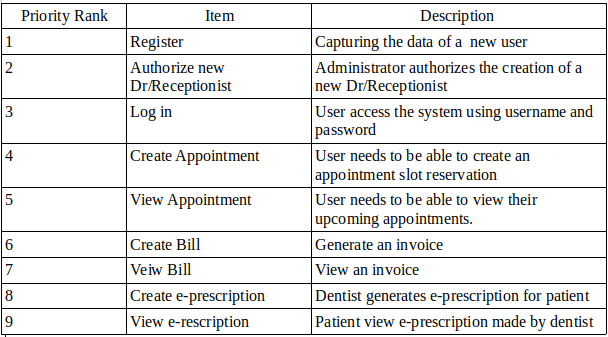
\includegraphics[width=\linewidth]{PriorityList.png}
\caption{Priority List}
\label{fig:ERD}
\end{figure}
\subsubsection{Sprint Backlog}
During the first sprint plan meeting, the product backlog was used to develop sprint backlogs.The first sprint comprises of 4 tasks/items. The tasks and their description are given below.
\begin{figure}[h]
\centering
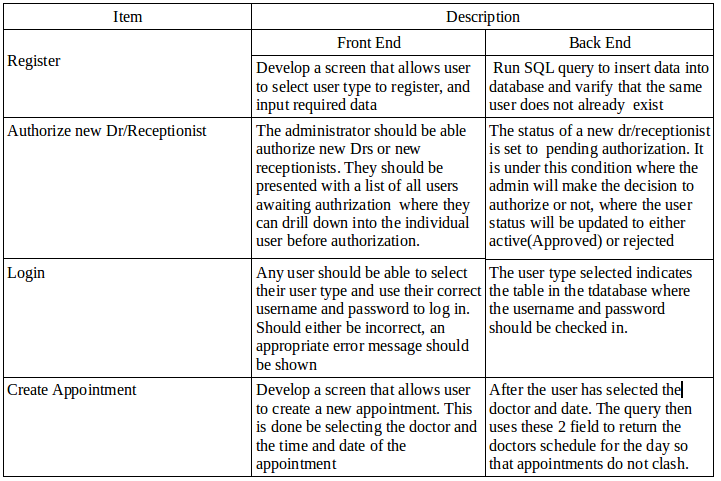
\includegraphics[width=\linewidth]{final.png}
\caption{Sprint 1}
\label{fig:ERD}
\end{figure}

\newpage
Each task was estimated to take at most 10 hrs.The first sprints ran for 5 days.Daily scrum meetings were conducted to check the progress of each team member and to unblock any impediments.At the end of each sprint, sprint review meetings were conducted to test and demonstrate the functionality of the product.A sprint burn down diagram which shows the progress of the first sprint is given below
\begin{figure}[h]
\centering
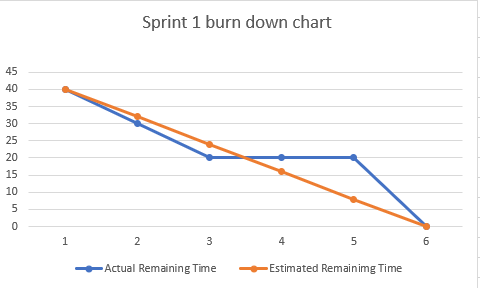
\includegraphics[width=\linewidth]{sprint1.PNG}
\caption{Sprint 1 burndown diagram}
\label{fig:ERD}
\end{figure}
\newpage
During the second sprint plan meeting, the product backlog was used to develop sprint backlogs.The second sprint comprises of 6 tasks/items. The tasks and their description are given below.

\newpage
\begin{figure}[h]
\centering
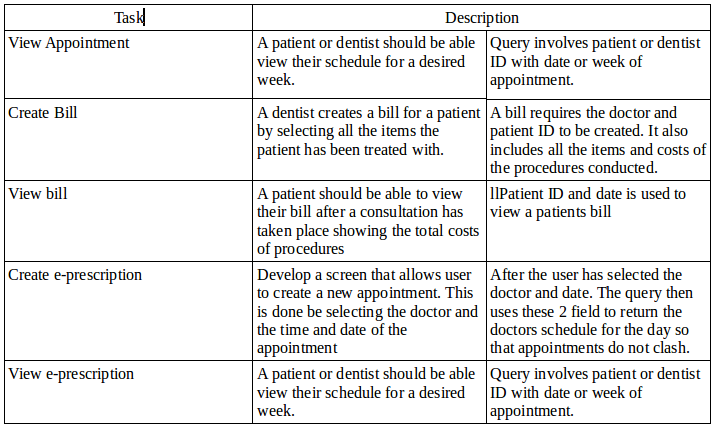
\includegraphics[width=\linewidth]{sprint2.png}
\caption{Sprint 2}
\label{fig:ERD}
\end{figure}

A second sprint of 5 tasks was formed from the product backlog.Each tasks was estimated to take at most 10 hrs and the sprint ran for 9 days.The tasks and their description are given below.A sprint burn down diagram which shows the progress of the second sprint is given below
\begin{figure}[h]
\centering
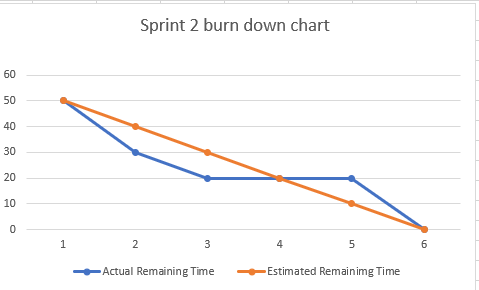
\includegraphics[width=\linewidth]{sprint3.PNG}
\caption{Burn down diagram}
\label{fig:ERD}
\end{figure}
\subsection{Sprint planning documents}

Sprint is timeboxed incremental iterations, each aims to produce a potentially shippable increment (PSI).\\
Product backlog(priority list)->after meeting sprint backlog breaking user story to tasks \\
Sprint 1 - User stories + Fixes for any outstanding bugs

Daily scrums - What has been done, sprint review meeting
followed by retrospective meeting
\clearpage
\section{Module Descriptions and Demonstrations}
\subsection{User login}
\begin{figure}[h]
\centering
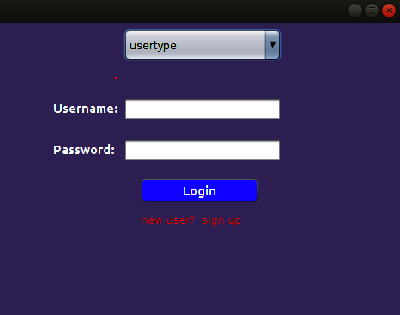
\includegraphics[width=0.7\linewidth]{login.png}
\caption{DCMS login}
\label{fig:login}
\end{figure}
All users are required to login before they can begin using the software's main capabilities. The user begins by selecting the user type which they are (Patient, Dentist, Receptionist or administrator). The entered username is then checked in the appropriate database table to see if the password entered matches the one stored. \\
The doctor's username is taken as the doctor's practice number, all other users use their email addresses as usernames.
Data validation is done on the screen to show appropriate error messages if anything is incorrect(refer to
\hyperref[sec:system_testing]{System Testing} )
\subsection{User Registration}
\begin{figure}[h]
\centering
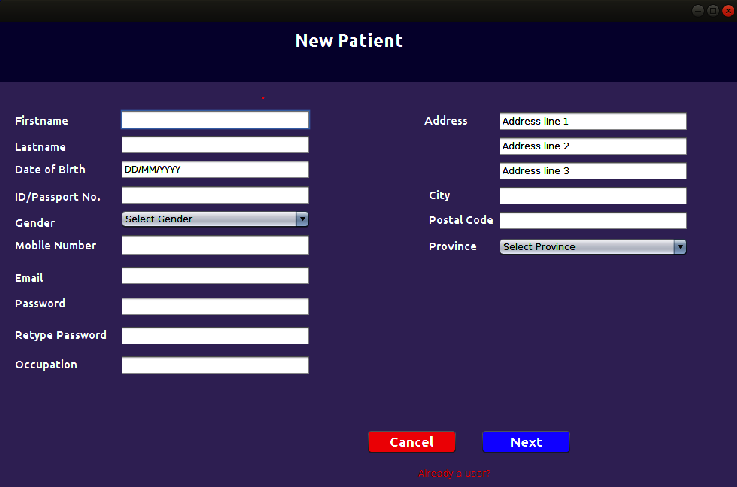
\includegraphics[width=\linewidth]{UI_create_ patient.png}
\caption{Create patient}
\label{fig:create_patient}
\end{figure}
Should the user be new and without a username and password, they are required to register as a new user. Based on the input of the combo box, the correct new user portal is loaded. The above the User Interface shows the registration of a new patient.
\begin{figure}[h]
\centering
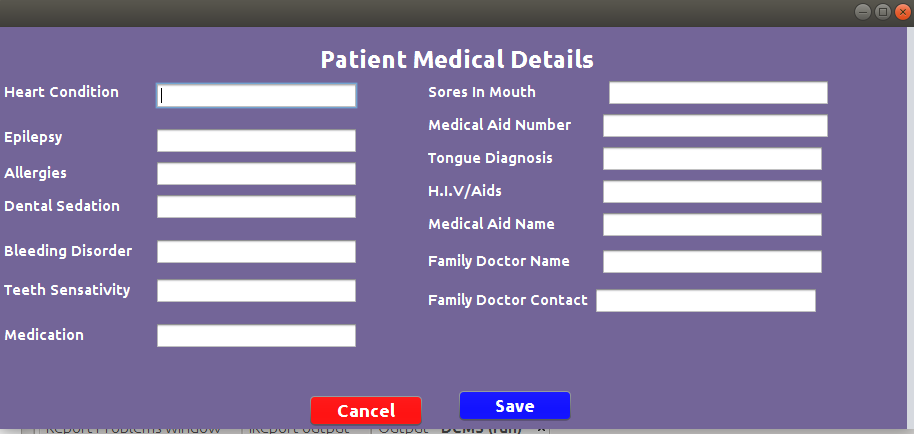
\includegraphics[width=\linewidth]{patientmedicalcond.png}
\caption{Create patient, medical details}
\label{fig:Patient Medical details}
\end{figure}
\begin{figure}[h]
\clearpage
\centering
\includegraphics[width=.6\linewidth]{"new dentist".png}
\caption{Create Dentist}
\label{fig:Create New Dentist}
\end{figure}
The above user interface shows the registration of a new dentist. The button on the top left (Authorize), is only clickable from the administrator point of view. After the dentist has entered all their required data, in order to be able to use the created credentials to log in, the new dentist must first be authorized(approved to be legitimate) by the administrator.

\begin{figure}[h]
\centering
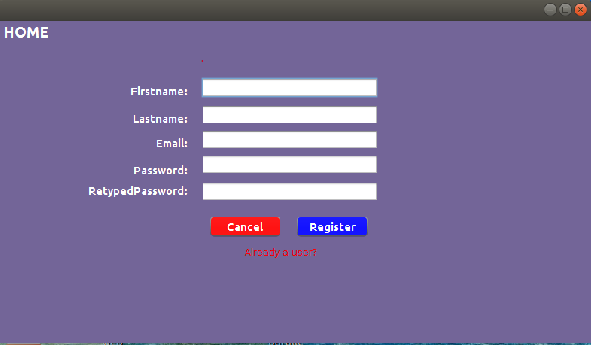
\includegraphics[width=\linewidth]{new_receptionist.png}
\caption{Create Receptionist}
\label{fig:Create New Receptionist}
\end{figure}
\clearpage
\subsection{Home Screens}
Below shows the different home screens seen by different user types after logging in, the current username is what appears in the top panel.
\begin{figure}[h]
\centering
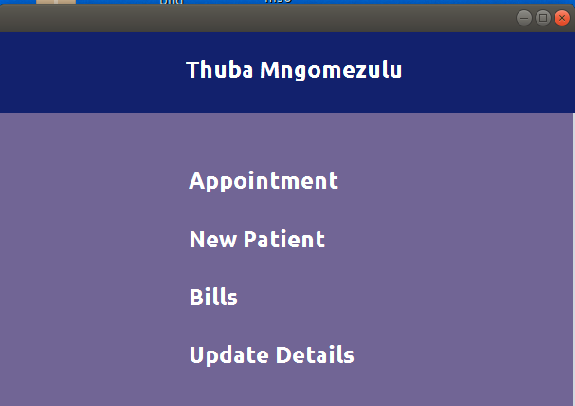
\includegraphics[width=.7\linewidth]{receptionist_home.png}
\caption{Receptionist Home Screen}
\label{fig:ERD}
\end{figure}
The receptionist has 4 possible options to click.
\begin{itemize}
\item
"Appointment" allows them to either view or create a new appointment for a patient. Patients can also call to cancel appointments
\item
"New Patient" takes them to the page a new patient can be registered.
\item
"Bills" takes a look at all invoices recorded for either a dentist or patient. This option can be used for patients without capabilities of using the system remotely and would like to either have the bill printed or sent in some other way. This is where all the financial management is done by the receptionist.
\item
"Update Details" Receptionist can update their own details ranging from personal details to password
\end{itemize}
\begin{figure}[h]
\centering
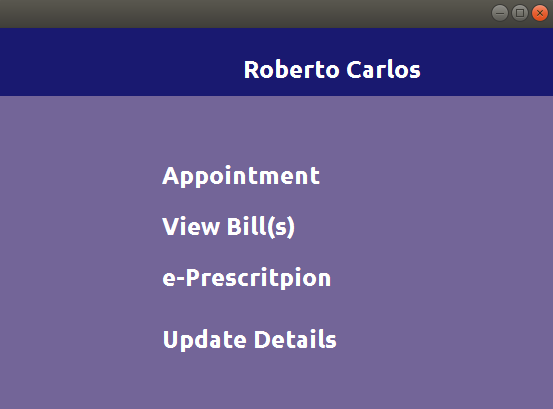
\includegraphics[width=.7\linewidth]{patient_home.png}
\caption{Patient Home Screen}
\label{fig:ERD}
\end{figure}
\begin{itemize}
\item
"Appointment"-A patient can either set, view or cancel appointment. Appointment cancellation is done to avoid being charged a missed appointment fees.
\item
"View Bill(s)" -This is where patients can view their bills. This offers them a breakdown of all costs from their past consultations.
\item
"Update Details" - Updating of any of their personal details, medical conditions or password.
\item
"Prescription" patient can view the e-prescription made by dentist. This can be shown to the pharmacist when collecting the medication.
\clearpage
\end{itemize}
\begin{figure}[h]
\centering
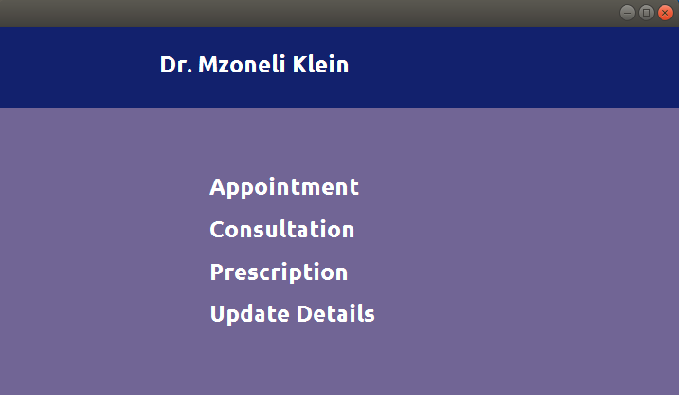
\includegraphics[width=.7\linewidth]{dr_home.png}
\caption{Dentist Home Screen}
\label{fig:ERD}
\end{figure}
\begin{itemize}
\item
"Appointment" A dentist can view their schedule for any given time.
\item
"Consultation" The dentist begins recording the medical procedures and the charges of each. This is what becomes the invoice or bill of the patient.
\item
"Prescription" Dentist creates an e-prescription for the patient.
\item
"Update Details" Dentist can update their personal details as well as password.
\end{itemize}
\clearpage
\subsection{Appointments}
\begin{figure}[h]
\centering
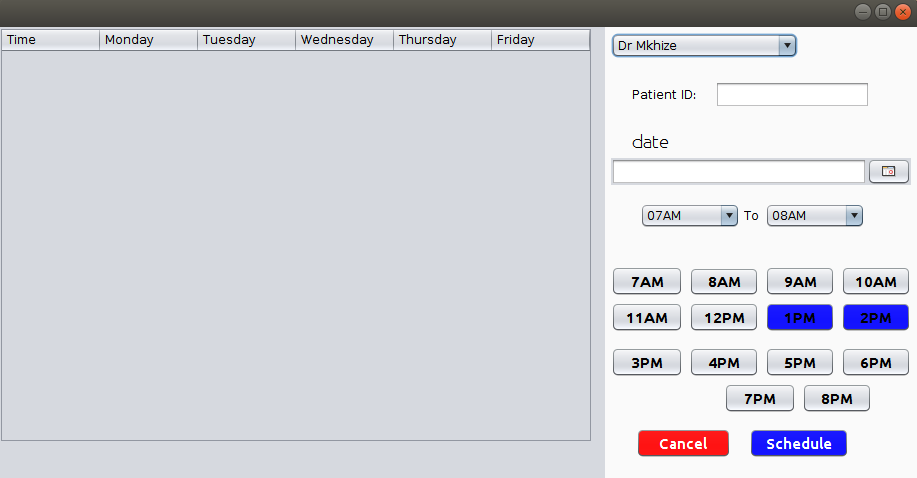
\includegraphics[width=\linewidth]{new_appointment.png}
\caption{Create Appointment}
\label{fig:Appointment}
\end{figure}
The creation of a new appointment can be done by either the patient or the receptionist. The details recorded include the patient making the booking and the doctor being booked for. Each patient has a prefered dentist, however one has the option of booking to see a different dentist who may have a different specialization for the needed appointments. \\
The appointment has a date and time selection, the dates available are from the schedule of the selected doctor for the given week. This is to ensure that appointments are not double booked for doctors. \\
Patients that arrive without prior booking who form part of the triage, are attended to by the receptionist. The receptionist can then allocate this patient an appointment right then and there where the dentist can also see in his own schedule that a new priority visit is in line.

\begin{figure}[h]
\centering
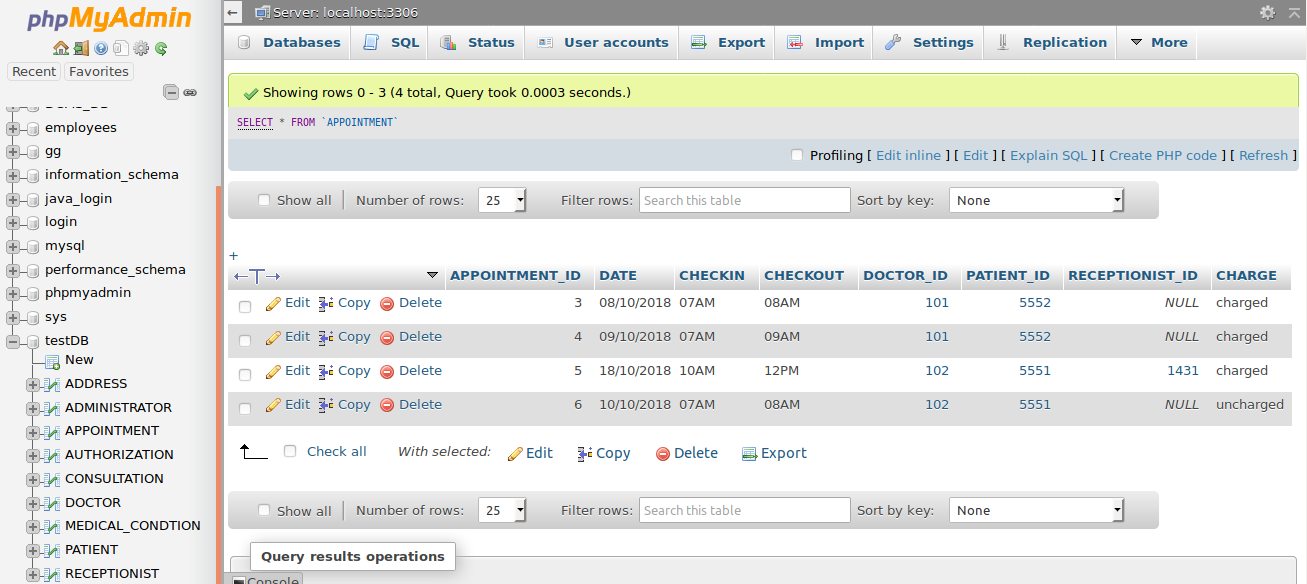
\includegraphics[width=\linewidth]{appointment_table_php.png}
\caption{Create Appointment}
\label{fig:Appointment}
\end{figure}
The illustration above shows how a new appointment is structure and stored. The phpMyAdmin tool is used for administering MySQL, and from the table extract above we can see that the appointment schedule details are captured from what is entered in the front end correctly.\\
Once an appointment has been set, dentists and patients can view their respective schedules from their portals on the system. A dentist can then select whichever appointment is next and begin recording the consultation as described below. \\

\subsection{Finance Management}
\begin{figure}[h]
\centering
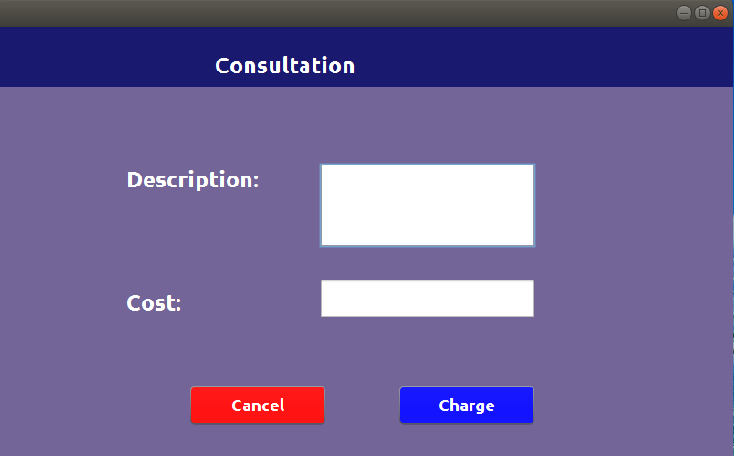
\includegraphics[width=0.6\linewidth]{consultation.png}
\caption{Create patient}
\label{fig:Add consultation procedure and cost}
\end{figure}
After a consultation has been conducted, the dentist or receptionist is then tasked with capturing the procedures and costs of what was done. The prices of procedures were found to be different from patient and thus we found that it was best to allow the dentists to enter the cost charged for each patient. Each description and cost can be thought of as a line of record that will appear on the bill or invoice.\\
Once all procedure items have been recorded and the bill is complete, the patient is then able to view their bill under their system portal. Within that page the dentist's payment details and conditions are displayed. When payments are made, the bill balance is updated.
\newpage

\section{System development review method}
\subsection{Sprint retrospective}
What went right:
\begin{itemize}
\item
The co-ordination of team members which was facilitated by the regular scrum meetings ensured that all team members were kept updated on progress and what still needed to be done
\item
The us
The use of GitHub for version control meant that all work done could be seen by all team members offering transparency and good project element integration.

\end{itemize}
What went wrong:
\begin{itemize}
\item The appointment user story was a lot bigger than expected. This user story should have been broken down into smaller sub stories. The process of checking the dentist schedule to make sure they'll be no clashes should have been given more priority.
\item
We initially planned to use lamp server to host the project. Due to the difficulty of connecting the database to the netbeans java project, this approach was left. It would have required the use of php and JSON file.
\item
The scrum meetings did not take place daily due to team members having other commitments during the project span. However we did meet regularly, not daily as scrum suggest.


\end{itemize}

\section{System Testing}
\subsection{Unit Tests}
Unit testing also called component testing was performed on standalone modules to check whether they were developed correctly. The following standalone modules were tested
\begin{itemize}
\item \textbf{Login}
\begin{figure}[h]
\centering
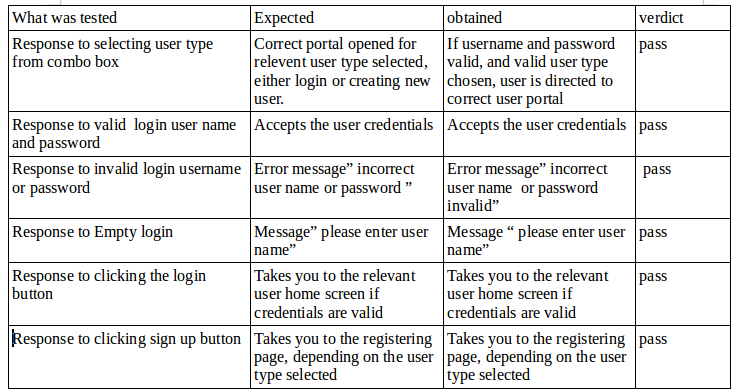
\includegraphics[width=\linewidth]{Logins.png}
\caption{login testing}
\label{fig:ERD}
\end{figure}
\newpage
\item \textbf{Register}
\begin{figure}[h]
\centering
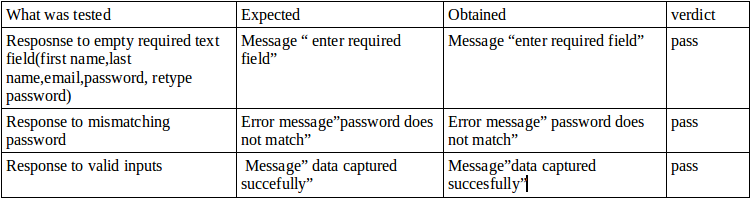
\includegraphics[width=\linewidth]{register.png}
\caption{Register testing}
\label{fig:ERD}
\end{figure}

\end{itemize}
The other components of the software were tested during the programming of the software. This approach can be thought of as a white-box approach. Checking the module integration by making sure that the correct user details are passed from screen to screen. Checking that the calculations of the the bill as part of the financial management to see that they were added correctly.
\end{document}




